\chapter{不对称合成}\label{ch:b3:asymmetric-synthesis}

L-DOPA 是一种缓解帕金森病症状的药物，它在
1970 年代是首个通过不对称催化工业化制得的化合物：仅需
数克手性铑配合物与一种平面、非手性的前体一起溶解，
在氢气中反应，所得产物中一种对映体远多于另一种。
药物的两种对映体，其作用可能截然不同，
因为它们所遇到的受体与酶本身就是手性的。本章
讨论对映体纯度的测定，说明手性环境如何在
两条互为镜像的路径之间进行选择，并介绍各类策略（手性源、
手性助剂、拆分、金属与有机催化剂）等，用以制备
单一对映体。

\begin{recall}
本科一年级分册定义了手性、对映体、非对映体、外消旋混合物、
比旋光度、CIP 规则，以及立体选择性反应与立体专一反应；
本科二年级分册讨论了催化氢化、环氧化、双羟基化、
亚胺、烯胺、烯醇负离子、羟醛反应、
罗宾逊成环与色谱法。\Cref{ch:b3:rate-theories}给出了
艾林方程，\cref{ch:b3:homogeneous-catalysis}给出了威尔金森循环，以及
\cref{ch:b3:point-groups}中的 $C_2$ 轴。
\end{recall}

\begin{omfigure}
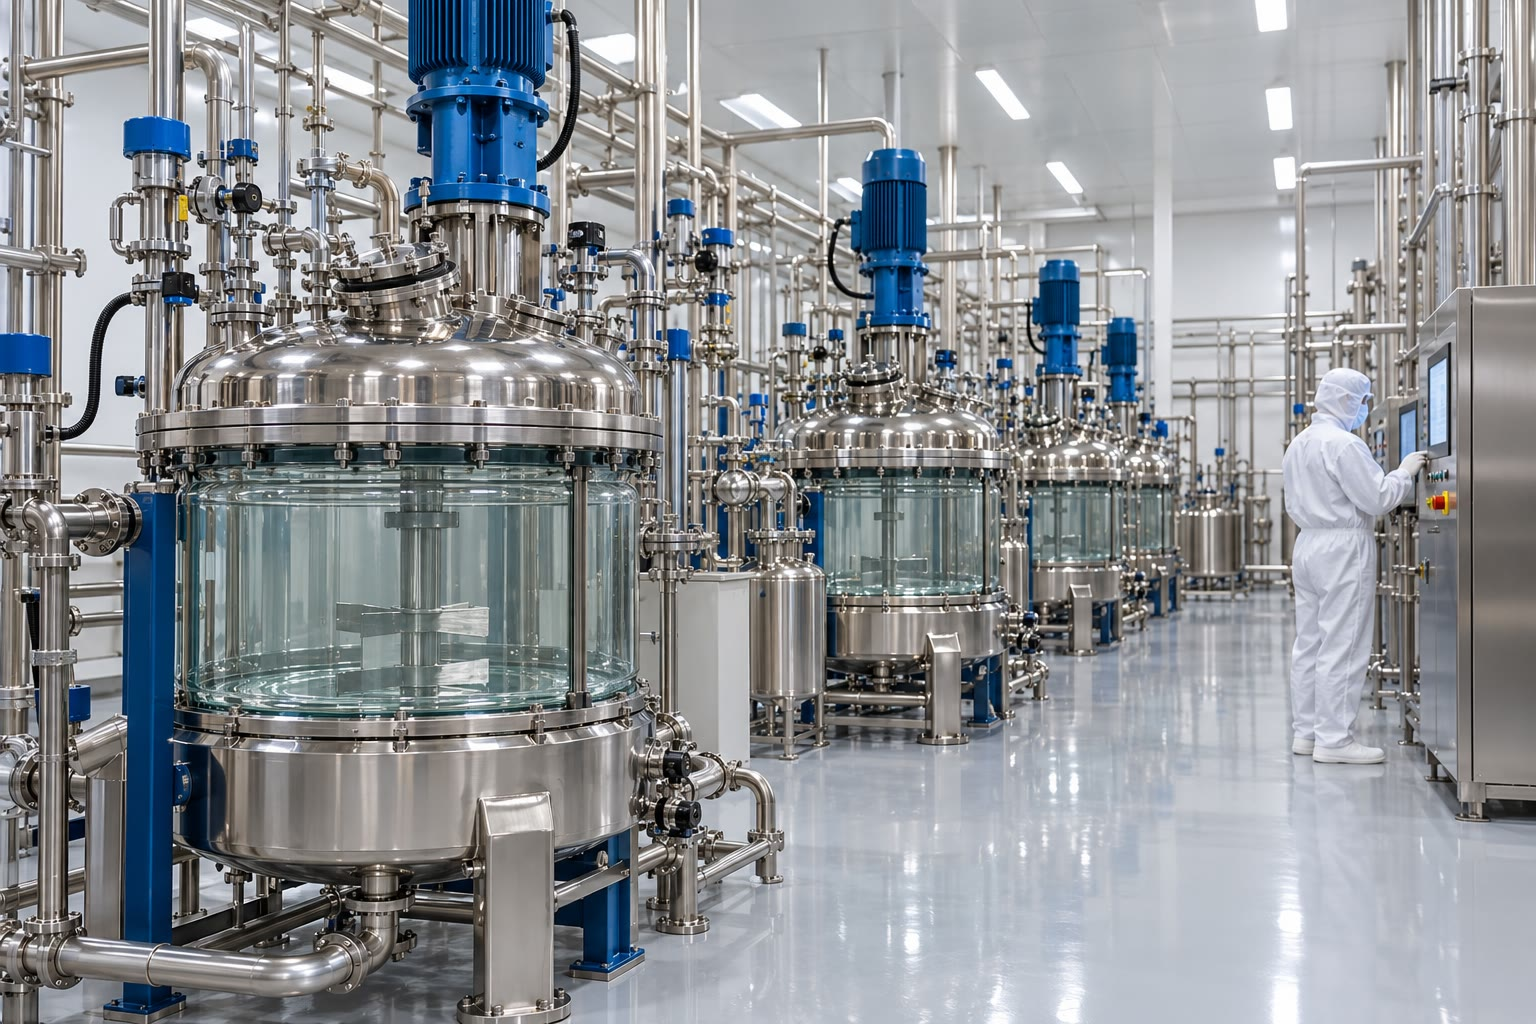
\includegraphics[width=0.58\linewidth]{images/book4/ai/b3-28-api-plant.jpg}

{\small 一座制造活性药物成分的工厂，车间内排列着搪玻璃反应釜。
其中许多产品为单一对映体，
通过催化或拆分制得，并以手性色谱法检测。}
\end{omfigure}

\section{对映体纯度的测定}

\begin{definition}[对映体过量]\label{def:b3:asymmetric-synthesis:ee}
对于物质的量分别为 $n_R \ge n_S$ 的对映体混合物，称\emph{对映体过量}
\index{对映体过量}为 $\mathrm{ee} = (n_R - n_S)/(n_R + n_S)$，称\emph{对映体比例}
\index{对映体比例} $\mathrm{er} = n_R/n_S$；对于非对映体，
\emph{非对映体过量}\index{非对映体过量}（de）的定义方式相同。
\emph{光学纯度}\index{光学纯度}是样品的
比旋光度与纯对映体比旋光度之比。
\end{definition}

\begin{proposition}[ee 与 er]\label{prop:b3:asymmetric-synthesis:ee-er}
$\mathrm{ee} = (\mathrm{er} - 1)/(\mathrm{er} + 1)$，且 $\mathrm{er} = (1 + \mathrm{ee})/(1 - \mathrm{ee})$。
\end{proposition}

\begin{proof}
将 $(n_R - n_S)/(n_R + n_S)$ 的分子与分母同除以 $n_S$，解出 er 即得
第二个式子。
\end{proof}

ee 为 90\,\% 时，er 为 95\,:\,5；ee 为 98\,\% 时，er 为 99\,:\,1。
光学纯度只有当旋光度与组成成正比时才等于 ee；杂质、
溶剂、浓度效应以及许多化合物的旋光很小，都会使其不可靠，
因此 ee 需通过分离对映体来测定。

\begin{method}[由手性色谱图求对映体过量]\label{met:b3:asymmetric-synthesis:ee-chromatogram}
\begin{enumerate}
  \item 先进样外消旋混合物，以确定两个峰并检查其
        分离度（基线分离）及峰面积是否相等。
  \item 进样待测样品，并对两个峰积分。
  \item 对映体在非手性检测器上的响应相同，因此
        $\mathrm{ee} = (A_1 - A_2)/(A_1 + A_2)$；用纯对映体标准品指认各峰。
\end{enumerate}
\end{method}

\begin{omfigure}
\begin{tikzpicture}
\begin{axis}[name=a, width=0.48\linewidth, height=5.4cm, xmin=0, xmax=20, ymin=0, ymax=1.0,
  axis lines=left, xlabel={$\Delta\Delta G^\ddagger$ / \unit{kJ.mol^{-1}}}, ylabel={对映体过量},
  tick label style={font=\scriptsize}, label style={font=\small}]
\addplot[omDef, thick] table[x=ddg, y=eeA] {figdata/out/bachelor-3-er-ddg.dat};
\addplot[omMeth, thick] table[x=ddg, y=eeB] {figdata/out/bachelor-3-er-ddg.dat};
\addplot[omThm, thick] table[x=ddg, y=eeC] {figdata/out/bachelor-3-er-ddg.dat};
\node[font=\scriptsize, omDef, anchor=west] at (axis cs:10,0.55) {\qty{-78}{\celsius}};
\node[font=\scriptsize, omMeth, anchor=west] at (axis cs:10,0.43) {\qty{0}{\celsius}};
\node[font=\scriptsize, omThm, anchor=west] at (axis cs:10,0.31) {\qty{25}{\celsius} （最低曲线）};
\end{axis}
\begin{axis}[at={(a.east)}, anchor=west, xshift=1.4cm, width=0.48\linewidth, height=5.4cm,
  xmin=7.5, xmax=9.5, ymin=0, axis lines=left, ytick=\empty,
  xlabel={保留时间 / min}, ylabel={检测器信号},
  tick label style={font=\scriptsize}, label style={font=\small}]
\addplot[black, thick] table[x=t, y=y] {figdata/out/bachelor-3-er-ddg-b.dat};
\node[font=\scriptsize, anchor=south west] at (axis cs:8.3,250) {(\textit{R}): 97.5};
\node[font=\scriptsize, anchor=south] at (axis cs:9.1,20) {(\textit{S}): 2.5};
\end{axis}
\end{tikzpicture}

{\small 左图为对映体过量随两条竞争路径的活化吉布斯自由能之差的变化，
给出三种温度下的结果：相同的
$\Delta\Delta G^\ddagger$ 在低温下给出更高的对映体过量。右图：手性 HPLC 色谱图，
峰面积分别为 97.5 与 2.5（模型）：对映体过量 95\,\%。}
\end{omfigure}

核磁共振只有在手性环境中才能区分对映体：手性溶剂化
试剂会形成寿命很短的非对映体配合物，使其信号有所不同；而手性醇或胺
与莫舍酸反应生成两种非对映体酯，
由位移差的模式即可判断构型。

\begin{method}[由莫舍酯判断构型（概要）]\label{met:b3:asymmetric-synthesis:mosher}
\begin{enumerate}
  \item 分别制备该醇的 (\textit{R})- 与 (\textit{S})-MTPA 酯。
  \item 记录两者的质子谱，并对与羟基相连碳原子两侧的每个质子计算
        $\Delta\delta = \delta_S - \delta_R$。
  \item 在优势构象中，酸的苯环屏蔽一侧：
        $\Delta\delta > 0$ 的质子位于一侧，$\Delta\delta < 0$ 的质子位于另一侧，
        由此确定两个取代基的位置，进而得出构型。
\end{enumerate}
\end{method}

\section{拓扑性与立体选择性加成}

\begin{definition}[立体选择性反应]\label{def:b3:asymmetric-synthesis:selective}
称\emph{对映选择性反应}\index{对映选择性反应}生成的产物中
一种对映体多于另一种；称
\emph{非对映选择性反应}\index{非对映选择性反应}生成一种非对映体占优。
\end{definition}

\begin{definition}[拓扑性]\label{def:b3:asymmetric-synthesis:topicity}
若分子的两个基团可经分子的旋转而互换，则称它们为\emph{等位的}\index{等位的}，
即替换其中任一基团得到同一化合物；
若仅可经反映互换，则称它们为\emph{对映异位的}\index{对映异位的}，
即替换其中任一基团得到对映体；并且
若任何对称操作都不能使二者互换，则称为\emph{非对映异位的}\index{非对映异位的}，
即替换其中任一基团得到非对映体。
\end{definition}

与手性中心相邻的 $\ce{CH2}$ 基团上的两个氢是非对映异位的：它们
化学位移不同且彼此耦合，这正是此类
基团在核磁共振谱中常呈现两组信号的原因。

\begin{definition}[前手性面]\label{def:b3:asymmetric-synthesis:faces}
连有三个不同取代基的三角形碳原子是\emph{前手性的}\index{前手性的}：
加入第四个不同基团即生成手性中心。从此面看去，
三个取代基按 CIP 优先级递减顺时针排列时，该面为
\emph{Re 面}\index{Re 面}；逆时针排列时，为\emph{Si 面}\index{Si 面}。
\end{definition}

\begin{omfigure}
\begin{tikzpicture}[font=\small, >=Stealth]
  \coordinate (c) at (0,0);
  \draw[thick, double, double distance=1.6pt] (c) -- (90:1.1) node[above] {O（1）};
  \draw[thick] (c) -- (210:1.1) node[below left] {$\ce{C6H5}$（2）};
  \draw[thick] (c) -- (330:1.1) node[below right] {$\ce{CH3}$（3）};
  \fill (c) circle (1.6pt);
  \draw[->, thick, omThm] (70:0.6) arc[start angle=70, end angle=200, radius=0.6];
  \node[font=\scriptsize, omThm, align=center] at (-1.9,0.75) {1 $\to$ 2 $\to$ 3\\ 逆时针：\\ \textit{Si} 面};
  \node[font=\scriptsize, align=left, anchor=west] at (2.6,0.4) {朝向读者的面为 \textit{Si} 面 \\ 纸背后的面为 \textit{Re} 面};
  \node[font=\scriptsize, align=left, anchor=west] at (2.6,-0.5) {从 \textit{Re} 面加入氢负离子 \\ 得到 (\textit{S})-1-苯基乙醇};
\end{tikzpicture}

{\small 苯乙酮的各面。从前方看，羰基碳原子上的取代基按 CIP 次序
（O、苯基、甲基）呈逆时针排列，前面为 \textit{Si} 面，
背面为 \textit{Re} 面。}
\end{omfigure}

\begin{method}[标注 Re 面与 Si 面]\label{met:b3:asymmetric-synthesis:re-si}
\begin{enumerate}
  \item 按 CIP 规则给三角形原子的三个取代基排序（
        双键按其另一端的原子计两次）。
  \item 观察所关注的面，即位于纸面内的三角形平面。
  \item 顺时针 1 $\to$ 2 $\to$ 3：\textit{Re}；逆时针：\textit{Si}。
  \item 命名产物时，将新基团加在朝向观察者的一侧，并对新手性中心应用
        CIP 规则；Re 面进攻并不总是得到 \textit{R} 构型。
\end{enumerate}
\end{method}

\begin{definition}[费尔金–安模型与螯合控制]\label{def:b3:asymmetric-synthesis:felkin}
\emph{费尔金–安模型}\index{费尔金–安模型}预测与手性中心相邻的
羰基亲核加成所得的主要非对映体：
该中心上最大的基团垂直于羰基平面，
亲核试剂从与之相反的一侧接近，越过最小的基团，
沿比尔吉–邓尼茨轨迹进攻。在\emph{螯合控制}\index{螯合控制}下，
一个金属离子同时与羰基氧及
手性中心上的给电子基团配位，从而锁定构象，亲核试剂
加到螯合环位阻较小的一面。
\end{definition}

\begin{proposition}[费尔金–安选择性]\label{prop:b3:asymmetric-synthesis:felkin}
对于不含螯合基团的 $\alpha$-手性醛或酮，主要产物为
费尔金–安模型所预测者（该模型为经验模型，
并得到计算支持）。\admitted
\end{proposition}

\begin{omfigure}
\begin{tikzpicture}[font=\small, >=Stealth]
  \foreach \a/\lab in {90/L, 330/M, 210/S} {
    \draw[line width=0.8pt] (\a:0.55) -- (\a:1.1) node[pos=1.3] {\lab};
  }
  \fill[white] (0,0) circle (0.55);
  \draw[line width=0.8pt] (0,0) circle (0.55);
  \draw[line width=0.8pt, double, double distance=1.4pt] (0,0) -- (0:1.1) node[right] {O};
  \draw[line width=0.8pt] (0,0) -- (180:1.1) node[left] {R};
  \draw[->, very thick, omThm] (250:2.2) -- (250:0.25);
  \node[omThm, anchor=north] at (250:2.25) {Nu$^-$};
  \node[font=\scriptsize, align=left, anchor=west] at (1.7,-1.0) {Nu$^-$ 从 L 的反侧进入，\\ 越过 S，\\ 与 C=O 键约成 107°};
\end{tikzpicture}

{\small 费尔金–安模型，沿羰基碳原子向手性中心的键方向观察（前方为羰基碳，
与 O 和 R 相连）；后方圆圈为手性中心，基团为 L、M 和 S。
较大的基团垂直于羰基平面；亲核试剂从
相反一侧接近，靠近较小的基团，远离氧原子。}
\end{omfigure}

\section{策略}

\begin{definition}[手性源]\label{def:b3:asymmetric-synthesis:chiral-pool}
\emph{手性源}\index{手性源}是一组廉价的、对映纯的
天然化合物（氨基酸、糖、萜类、羟基酸），用作
起始原料，其手性中心被带入目标分子。
\end{definition}

\begin{definition}[手性助剂]\label{def:b3:asymmetric-synthesis:auxiliary}
\emph{手性助剂}\index{手性助剂}是一种对映纯的基团，
暂时连接于底物上，用以控制
反应的立体化学，之后除去并回收。
\end{definition}

在埃文斯烷基化反应中，由氨基酸制得的噁唑烷酮被酰化；
锂或钠的烯醇负离子与助剂的羰基螯合，
在远离助剂取代基的一面被卤代烷进攻，
生成一种非对映体，通常 de 值高于 95\,\%；水解随后释放出
手性酸和助剂。

\begin{definition}[拆分]\label{def:b3:asymmetric-synthesis:resolution}
\emph{外消旋体拆分}\index{外消旋体拆分}是将其
分离为对映体，经典方法是使非对映异构体盐结晶，
所用的盐由对映纯的酸或碱形成。在\emph{动力学拆分}\index{动力学拆分}中，
两种对映体与手性试剂或催化剂以不同速率反应，
选择性为 $s = k_{\mathrm{fast}}/k_{\mathrm{slow}}$。在
\emph{动态动力学拆分}\index{动态动力学拆分}中，底物的两种对映体
快速互变，同时其中一种发生反应。
\end{definition}

\begin{theorem}[卡甘方程]\label{thm:b3:asymmetric-synthesis:kagan}
对于外消旋体的动力学拆分，若两个一级反应的选择性为 $s$，
转化率 $c$ 与剩余底物的 ee 满足关系：
\[
  s = \frac{\ln[(1 - c)(1 - \mathrm{ee})]}{\ln[(1 - c)(1 + \mathrm{ee})]}.
\]
\end{theorem}

\begin{proof}
每种对映体按指数规律衰减：剩余分数为 $f_1 = \eu^{-k_{\mathrm{fast}}t}$ 和
$f_2 = \eu^{-k_{\mathrm{slow}}t}$，故 $\ln f_1 = s\ln f_2$。由等量出发，$1 - c = (f_1 + f_2)/2$ 及
$\mathrm{ee} = (f_2 - f_1)/(f_1 + f_2)$。于是 $(1 - c)(1 - \mathrm{ee}) = \tfrac12(f_1 + f_2)\cdot 2f_1/(f_1 + f_2) = f_1$，类似地
$(1 - c)(1 + \mathrm{ee}) = f_2$。因此 $s = \ln f_1/\ln f_2$ 即为所述的比值。
\end{proof}

\begin{omfigure}
\begin{tikzpicture}
\begin{axis}[width=0.62\linewidth, height=5.6cm, xmin=0, xmax=1, ymin=0, ymax=1.02,
  axis lines=left, xlabel={转化率 $c$}, ylabel={ee},
  tick label style={font=\scriptsize}, label style={font=\small},
  legend style={font=\scriptsize, draw=none, at={(1.04,0.5)}, anchor=west}, legend cell align=left]
\addplot[color=omThm, thick] table[x=c, y=eesm] {figdata/out/bachelor-3-kinetic-resolution-s2.dat};
\addlegendentry{$s = 2$}
\addplot[color=omMeth, thick] table[x=c, y=eesm] {figdata/out/bachelor-3-kinetic-resolution-s10.dat};
\addlegendentry{$s = 10$}
\addplot[color=omDef, thick] table[x=c, y=eesm] {figdata/out/bachelor-3-kinetic-resolution-s50.dat};
\addlegendentry{$s = 50$}
\addplot[color=omThm, thick, dashed] table[x=c, y=eep] {figdata/out/bachelor-3-kinetic-resolution-s2.dat};
\addplot[color=omMeth, thick, dashed] table[x=c, y=eep] {figdata/out/bachelor-3-kinetic-resolution-s10.dat};
\addplot[color=omDef, thick, dashed] table[x=c, y=eep] {figdata/out/bachelor-3-kinetic-resolution-s50.dat};
\end{axis}
\end{tikzpicture}

{\small 动力学拆分：剩余底物（实线）与产物（虚线）的 ee 随转化率的变化，
取三种选择性。只要反应进行得足够远，底物总可以制成对映纯的，
但要以产率为代价；
产物在转化率低时最纯。}
\end{omfigure}

\begin{proposition}[动态动力学拆分]\label{prop:b3:asymmetric-synthesis:dkr}
若底物的两种对映体互变远快于任一种发生反应，
则整个外消旋体可以转化为一种产物对映体，其对映体比例由 $s$ 决定：
$\mathrm{er} = s$.
\end{proposition}

\begin{proof}
快速外消旋化使两种底物对映体在任何时刻
都保持等量。产物随后以速率比 $k_{\mathrm{fast}}[\mathrm A] : k_{\mathrm{slow}}[\mathrm A] = s$ 生成，且没有任何因素
会在底物（主要通过快速对映体）全部被消耗之前终止反应：
产率可达 100\,\%，对映体比例为 $\mathrm{er} = s$。
\end{proof}

\begin{method}[选择策略]\label{met:b3:asymmetric-synthesis:strategy}
\begin{enumerate}
  \item 若目标分子的手性碳原子存在于廉价的天然化合物中，
        则从手性源出发。
  \item 对于一次性合成，或要可靠地在羰基旁设定手性碳原子，
        则使用手性助剂，代价是多两步反应。
  \item 若外消旋体廉价，且不需要的对映体可以回收，或
        使其外消旋化，则拆分之（可用经典、动力学或动态动力学方法）。
  \item 若要大规模生产，应寻找不对称催化剂：
        每次催化周转生成一个手性碳原子，且不产生化学计量的手性废料。
\end{enumerate}
\end{method}

\section{金属的不对称催化}

\begin{definition}[不对称催化]\label{def:b3:asymmetric-synthesis:asymmetric-catalysis}
\emph{不对称催化}\index{不对称催化}是以少量手性催化剂进行的对映选择性
合成；对于金属催化剂，手性通常来自一个
\emph{手性配体}\index{手性配体}。
\end{definition}

\begin{theorem}[由能量得到的选择性]\label{thm:b3:asymmetric-synthesis:er-ddg}
若两种对映异构产物经由非对映过渡态生成，
且指前因子相等、反应不可逆、处于动力学控制之下，
则 $\mathrm{er} = \exp(\Delta\Delta G^\ddagger/RT)$，其中 $\Delta\Delta G^\ddagger$ 是两者
活化吉布斯自由能之差。
\end{theorem}

\begin{proof}
由艾林方程（见\cref{ch:b3:rate-theories}），
$k_i = (k_BT/h)\eu^{-\Delta G_i^\ddagger/RT}$；两种产物由同一反应物生成，故在每一时刻
其速率之比为 $k_1/k_2 = \eu^{(\Delta G_2^\ddagger - \Delta G_1^\ddagger)/RT}$，生成量之比亦然。
\end{proof}

在 \qty{25}{\celsius} 下，ee 为 99\,\%（er 为 199）需要 $\Delta\Delta G^\ddagger = RT\ln 199 = \qty{13.1}{kJ/mol}$，约相当于一个
氢键的能量；在 \qty{-78}{\celsius} 下，\qty{8.6}{kJ/mol} 即已足够。

\begin{proposition}[$C_2$ 对称配体]\label{prop:b3:asymmetric-synthesis:c2}
一个 $C_2$ 对称的手性配体使需要比较的非对映过渡态
数目减半，因为它留下的两个配位位点
是等价的。
\end{proposition}

\begin{proof}
催化剂的 $C_2$ 旋转把一个空位点映射到另一个，并使
催化剂保持不变。因此，一个位点上的任一过渡态与
另一位点上旋转所得的过渡态相同，只需比较一个位点上的结合方式（底物的面、
取向）需要比较。
\end{proof}

诺尔斯先用手性单膦配体，后用 $C_2$ 对称的双膦配体 DIPAMP，与铑配合，
将烯酰胺氢化为 L-DOPA 的受保护氨基酸；野依的 BINAP，
与钌配合，可氢化酮类和官能化烯烃，并且，
与手性二胺配合时，可以很高的对映体过量氢化简单酮。在
铑催化的烯酰胺氢化中，主要产物来自较不稳定的、
次要的催化剂–底物配合物，该配合物与氢气反应快得多：选择性
由过渡态决定，而非由中间体的布居数决定
（即柯廷–哈米特原理）。

\begin{definition}[夏普莱斯环氧化]\label{def:b3:asymmetric-synthesis:sharpless}
\emph{夏普莱斯环氧化}\index{夏普莱斯环氧化}是指
以叔丁基过氧化氢为氧化剂，对烯丙醇进行的对映选择性环氧化，
以异丙氧基钛（IV）催化，并配以对映纯的酒石酸二乙酯；
醇与钛结合，由钛把氧传递到烯烃的一个面上，
该面由酒石酸酯选定。
\end{definition}

\begin{omfigure}
\begin{tikzpicture}[font=\small, >=Stealth]
  \draw[black!50] (-2.3,-1.55) rectangle (2.5,1.55);
  % C3 (top) = C2 (bottom); C2 carries R1 (left) and CH2OH (lower right),
  % C3 carries R2 (left) and R3 (right)
  \coordinate (c3) at (0,0.45); \coordinate (c2) at (0,-0.45);
  \draw[thick, double, double distance=1.6pt] (c3) -- (c2);
  \draw[thick] (c3) -- (-0.9,0.95) node[above left, inner sep=1pt] {R$^2$};
  \draw[thick] (c3) -- (0.9,0.95) node[above right, inner sep=1pt] {R$^3$};
  \draw[thick] (c2) -- (-0.9,-0.95) node[below left, inner sep=1pt] {R$^1$};
  \draw[thick] (c2) -- (0.9,-0.95) node[below right, inner sep=1pt] {$\ce{CH2OH}$};
  \draw[->, very thick, omDef] (0.35,2.5) -- (0.2,0.1) node[pos=0, above, align=center, font=\scriptsize] {D-($-$)-酒石酸二乙酯：\\ O 来自上面};
  \draw[->, very thick, omThm] (0.35,-2.6) -- (0.2,-0.1) node[pos=0, below, align=center, font=\scriptsize] {L-($+$)-酒石酸二乙酯：\\ O 来自下面};
\end{tikzpicture}

{\small 夏普莱斯助记法。烯丙醇画在纸面上，
$\ce{CH2OH}$ 基团在右下方，L-($+$)-酒石酸二乙酯使氧从
纸面下方转移，D-($-$)-酒石酸二乙酯则从上方转移，无论
取代基 $\mathrm R^1$ 至 $\mathrm R^3$ 如何。}
\end{omfigure}

同样的思路，即金属被一种廉价的天然配体固定在手性口袋中，
得到以锇和金鸡纳生物碱配体催化的夏普莱斯烯烃不对称双羟基化。
当配体并非对映纯时，产物的对映体过量
未必与配体的成正比：两个配体组成的聚集体对同手性与异手性配对的活性不同，
会产生非线性效应，
有时是有益的放大。

\section{有机催化}

\begin{definition}[有机催化]\label{def:b3:asymmetric-synthesis:organocatalysis}
\emph{有机催化}\index{有机催化}是指
以不含金属的小分子有机物为催化剂的催化。在\emph{烯胺催化}\index{烯胺催化}中，
仲胺将酮或醛转化为亲核性烯胺；在
\emph{亚胺正离子催化}\index{亚胺正离子催化}中，将 $\alpha,\beta$-不饱和醛
转化为亲电性亚胺正离子，其 LUMO 能级降低。
\end{definition}

\begin{omfigure}
\begin{tikzpicture}[font=\small]
  % proline-derived enamine and the aldehyde held by the carboxylic acid
  \coordinate (n) at (0,0.7); \coordinate (r2) at (0.67,0.22); \coordinate (r3) at (0.41,-0.57);
  \coordinate (r4) at (-0.41,-0.57); \coordinate (r5) at (-0.67,0.22);
  \draw[thick] (n) -- (r2) -- (r3) -- (r4) -- (r5) -- (n);
  \node[fill=white, inner sep=0.6pt] at (n) {N};
  \coordinate (ca) at (0,1.45); \coordinate (cb) at (0.72,1.85);
  \draw[thick] (0,0.88) -- (ca);
  \draw[thick] (ca) -- (-0.62,1.85) node[left, inner sep=1pt] {$\ce{CH3}$};
  \draw[thick, double, double distance=1.5pt] (ca) -- (cb);
  \coordinate (cacid) at (1.45,0.45);
  \draw[thick] (r2) -- (cacid);
  \draw[thick, double, double distance=1.5pt] (cacid) -- (1.75,-0.15) node[below, inner sep=1pt] {O};
  \draw[thick] (cacid) -- (2.05,0.9) node[right, inner sep=1pt] (oh) {O--H};
  \node (cald) at (1.55,2.55) {C};
  \draw[thick, double, double distance=1.5pt] (cald) -- (2.35,2.15) node[right, inner sep=1pt] (oald) {O};
  \draw[thick] (cald) -- (1.3,3.15) node[above, inner sep=1pt] {R};
  \draw[omThm, thick, densely dashed] (cb) -- (cald);
  \draw[omMeth, thick, dotted] (2.45,1.05) -- (2.5,2.0);
  \node[font=\scriptsize, omThm, anchor=east] at (1.05,2.35) {C--C 成键};
  \node[font=\scriptsize, omMeth, anchor=west] at (2.6,1.55) {氢键};
\end{tikzpicture}

{\small 脯氨酸催化羟醛反应的示意过渡态：由丙酮与吡咯烷氮原子生成的
烯胺进攻醛，
醛的氧通过氢键与催化剂的羧酸结合，
该氢键决定醛的哪个面被进攻。}
\end{omfigure}

脯氨酸是一种廉价的氨基酸，能以高对映体过量催化三酮的分子内
羟醛反应（哈约斯–帕里什酮和维兰德–米歇尔酮，自 1970 年代起用于甾体合成），
并且，2000 年的研究表明，丙酮与醛的分子间
羟醛反应也可进行。手性咪唑烷酮通过亚胺正离子
参与第尔斯–阿尔德反应与共轭加成；手性
磷酸是具有手性口袋的强布朗斯特酸，通过质子化活化亚胺。
有机催化剂对空气和水稳定，
且产物中不残留金属。

\begin{inthelab}[手性 HPLC 分析]
手性色谱柱为涂有纤维素或直链淀粉衍生物的硅胶，
以己烷–异丙醇混合溶剂平衡。先注入外消旋混合物，
调节溶剂比例，直至两峰基线分离；然后
将样品溶于洗脱剂，浓度约每毫升一毫克，随后注入
并在两者均有吸收的波长处对峰进行积分。
\end{inthelab}

\begin{safety}{\ghs[0.6cm]{GHS02}\ghs[0.6cm]{GHS05}\ghs[0.6cm]{GHS06}\ghs[0.6cm]{GHS08}\ghs[0.6cm]{GHS09}}
% ledger: ghs4:TBHP, ghs4:TiOiPr4
叔丁基过氧化氢：易燃，受热时易自身反应，与皮肤接触有毒，
有腐蚀性，有致敏性，怀疑可致遗传缺陷；使用时
以溶液形式使用，低温保存，切勿浓缩，过量的过氧化物需
在后处理前销毁。异丙氧基钛（IV）：易燃，有刺激性，遇
湿气分解。
\end{safety}

\begin{history}[非对称催化的两项诺贝尔奖]
威廉·诺尔斯、野依良治和巴里·夏普莱斯因
手性催化的氢化与氧化反应，共同获得 2001 年诺贝尔化学奖。本杰明·利斯特和
戴维·麦克米兰曾于 2000 年证明，小的有机分子
能够像金属配合物一样广泛地催化对映选择性反应，
二人于 2021 年获得诺贝尔化学奖。
\end{history}

\section{练习}

\begin{exercise}[$\star$]\label{exo:b3:asymmetric-synthesis:1}
换算：ee 为 80\,\% 时的 er；er 为 99\,:\,1 时的 ee；
ee 为 50\,\% 时各对映体的百分含量。
\end{exercise}

\begin{exercise}[$\star$]\label{exo:b3:asymmetric-synthesis:2}
某手性 HPLC 谱图中，两个对映体的峰面积分别为 1840 和 60。
计算 ee。
\end{exercise}

\begin{exercise}[$\star$]\label{exo:b3:asymmetric-synthesis:3}
指出丙醛羰基碳的 Re 面和 Si 面，
并命名甲基亲核试剂从 Re 面加成所生成的醇。
\end{exercise}

\begin{exercise}[$\star$]\label{exo:b3:asymmetric-synthesis:4}
乙醇中两个亚甲基质子是等位的、对映异位的还是非对映异位的？
2-丁醇中 $\ce{CH2}$ 基团的两个质子又如何？
\end{exercise}

\begin{exercise}[$\star\star$]\label{exo:b3:asymmetric-synthesis:5}
求达到 99\,\% ee 所需的 $\Delta\Delta G^\ddagger$，分别在 \qty{25}{\celsius} 和 \qty{-78}{\celsius} 下计算，
并求在 \qty{-78}{\celsius} 下，一种在 \qty{25}{\celsius} 时给出 80\,\% ee 的催化剂（取相同的 $\Delta\Delta G^\ddagger$）所能给出的 ee。
\end{exercise}

\begin{exercise}[$\star\star$]\label{exo:b3:asymmetric-synthesis:6}
某胺样品的 $[\alpha]_D = -12.0$，在同样条件下纯的 (\textit{S})
对映体为 $-15.0$（练习给定数据）。求其光学纯度及各对映体的
百分含量，假设旋光度与组成成正比。
为何该测量不如色谱法可靠？
\end{exercise}

\begin{exercise}[$\star\star$]\label{exo:b3:asymmetric-synthesis:7}
在脂肪酶催化的外消旋醇乙酰化反应中，剩余醇
在转化率为 60\,\% 时的 ee 为 90\,\%。计算 $s$。
\end{exercise}

\begin{exercise}[$\star\star$]\label{exo:b3:asymmetric-synthesis:8}
预测 (\textit{E})-己-2-烯-1-醇分别与 L-($+$)-酒石酸二乙酯和
D-($-$)-酒石酸二乙酯反应所生成的环氧化物。
\end{exercise}

\begin{exercise}[$\star\star$]\label{exo:b3:asymmetric-synthesis:9}
(\textit{S})-2-苯基丙醛与甲基溴化镁反应。用费尔金–安模型
预测主要的非对映异构体。
\end{exercise}

\begin{exercise}[$\star\star\star$]\label{exo:b3:asymmetric-synthesis:10}
证明：在动力学拆分中，低转化率时产物的 ee 趋于 $(s - 1)/(s + 1)$，
并对 $s = 20$ 计算该值。为何动力学拆分更适合纯化底物，
而不是制备产物？
\end{exercise}

\begin{exercise}[$\star\star\star$]\label{exo:b3:asymmetric-synthesis:11}
羰基旁边含有可发生外消旋化的手性中心的酮，被
$s = 99$ 的酶还原，同时外消旋化很快。能达到何种产率和 ee？
与同一种酶在无外消旋化的情况下相比，
并在转化率为 50\,\% 时终止。
\end{exercise}

\begin{exercise}[$\star\star\star$]\label{exo:b3:asymmetric-synthesis:12}
运用柯廷–哈梅特原理解释：次要的催化剂–底物络合物如何
能够生成主要产物，其中两个络合物处于平衡
（有利于 A，$K = 10$），并以 $k_B/k_A = 600$ 反应。
\end{exercise}

\section{问题：L-DOPA 路线}

\begin{problem}[{周末问题——L-DOPA 路线：前手性烯酰胺及其
面、产生 95\,\% ee 的能量、通过结晶纯化，以及
动力学拆分需要什么}]
\label{pb:b3:asymmetric-synthesis:1}
% ledger: const:R
题目数据：铑催化的烯酰胺
前体在 \qty{25}{\celsius} 下氢化，得到 95\,\% ee 的受保护 (\textit{S})-氨基酸。
粗产物 100 克经重结晶：母液保留了全部次要
对映体，以及 5.0 克主要对映体。

\medskip\noindent\textbf{第一部分——底物。}
\begin{enumerate}
  \item 烯酰胺为何是前手性的？哪个碳成为手性中心？
  \item 若用非手性催化剂，会得到什么？
  \item 烯上的酰胺基团对催化剂为何重要？
  \item 手性双膦配体起什么作用？
  \item 主要产物是否由更稳定的催化剂–底物
        络合物生成？
  \item 为何在每个络合物中氢只加到一个面上？
\end{enumerate}

\medskip\noindent\textbf{第二部分——能量。}
\begin{enumerate}[resume]
  \item 求 95\,\% ee 对应的 er。
  \item 计算 $\Delta\Delta G^\ddagger$ 在 \qty{25}{\celsius} 时的值。
  \item 相同的 $\Delta\Delta G^\ddagger$ 在 \qty{-78}{\celsius} 时给出多大的 ee？
  \item 若 $\Delta\Delta G^\ddagger$ 增大 \qty{2}{kJ/mol}，在 \qty{25}{\celsius} 时给出多大的 ee？
  \item 将 \qty{9}{kJ/mol} 与氢键的能量相比较，并加以评论。
  \item 为何不直接把反应温度降低？
\end{enumerate}

\medskip\noindent\textbf{第三部分——结晶。}
\begin{enumerate}[resume]
  \item 计算粗产物中两个对映体的质量。
  \item 计算晶体的质量和 ee。
  \item 计算结晶的产率。
  \item 为何结晶可以提高样品的 ee，却永远无法从一个
        外消旋混合物中产生 ee（对于以外消旋化合物形式结晶的化合物）？
  \item 如何检验最终的 ee？
\end{enumerate}

\medskip\noindent\textbf{第四部分——改用动力学拆分。}
\begin{enumerate}[resume]
  \item 简单动力学拆分所能得到的一种对映体的最大产率是多少？
  \item 计算转化率为 55\,\% 时使剩余底物达到 95\,\% ee 所需的 $s$。
  \item 剩余底物的产率是多少？
  \item 动态动力学拆分会如何改变产率？
  \item 为何非对称氢化是更好的工业选择？
  \item 为何必须从药物中除去铑，以及如何测定？
  \item 写出结论：在 \qty{25}{\celsius} 下达到 95\,\% ee 所需的 $\Delta\Delta G^\ddagger$。
\end{enumerate}
\end{problem}
